Oscilační metody byly poprvé použity v 60.~letech 20.~století.  \cite{Cap2000} Zpočátku byla tato metoda pouze monofrekvenční, později byl použit pravoúhlý elektrický signál obsahující všechny frekvence, dnes se používá sada vhodně zvolených frekvencí. Význam a růst využití této metody koreloval s~technickými pokroky ve vývoji výpočetní techniky. První zkušenosti s~touto metodou v České republice se datují ke konci 90.~let. 

\subsection{Spirometrie}
Spirometrie je diagnostická metoda pro měření ventilace respiračního systému. Je založena na měření tlaku na síťce uvnitř spirometru, který je úměrný objemu vzduchu. \cite{MEFANET} Základním fyzikálním principem je analogie Ohmova zákona, kdy ze~zná\-mé\-ho průtoku vzduchu, tj obdoba proudu a známé překážky, tj obdobě odporu je vypočtena změna tlaku, tj obdoba napětí. Spirometr zaznamenává výsledek jako graf ukazující objem plic v~závislosti na čase. \cite{Medicon} Spirometrie je určena pro měření statických a dynamických parametrů plic. Statický parametr  je velikost alveolárního prostoru, která informuje o případných restrikčních poruchách, příkladem je dechový objem, inspirační rezervní objem nebo vitální kapacita. Dynamický parametr je průběh proudění vzduchu v dýchacích cestách, který informuje o obstrukčních poruchách. Příkladem je časová vitální kapacita, maximální výdechový proud vzduchu nebo maximální volní ventilace. \cite{lekfak}
Spirometrie je v praxi velmi rozšířená diagnostická metoda i přes její základní nedostatek, kdy plíce jsou měřeny jako jeden globální systém a tudíž spirometrie není schopna rozlišit ve které části plic se nachází potenciální patologie.
\begin{figure}[!ht]
			\centering
 			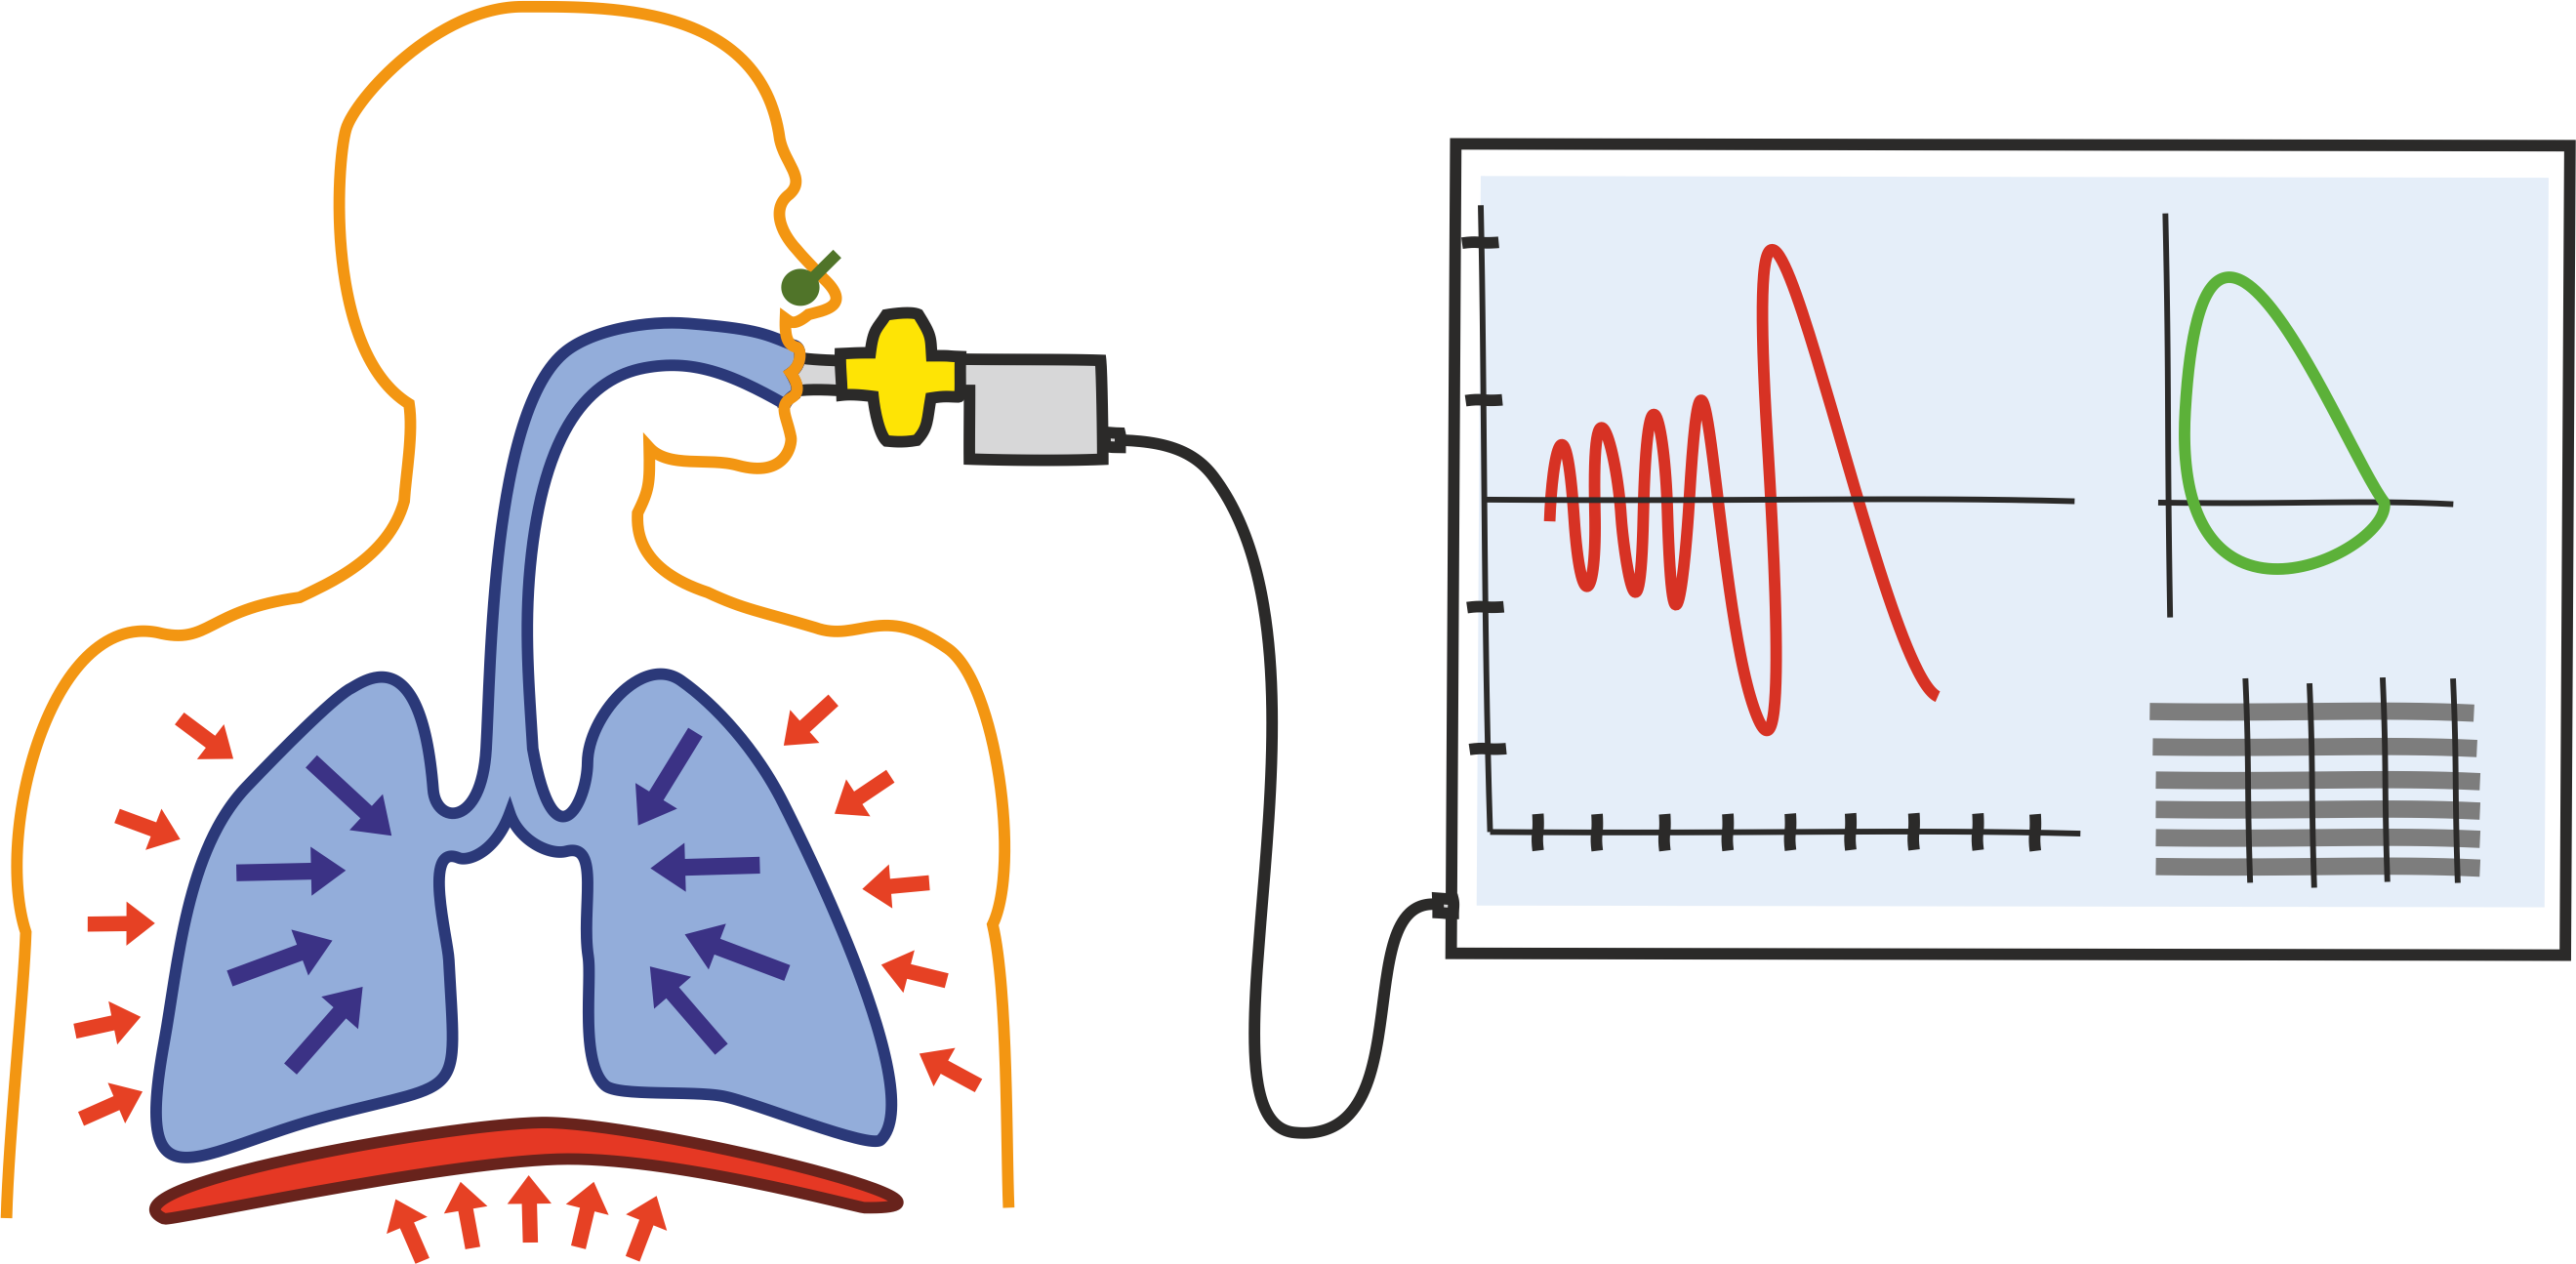
\includegraphics[width=1\textwidth]{spirometrie-wiki}
			\caption{Spirometrické vyšetření \cite{spirowiki}}
			 \label{vysetreni}
 \end{figure}

\subsection{Metoda nucených oscilací}
Metoda nucených oscilací je novější diagnostická metoda měření ventilace respiračního systému. Funguje na podobném principu jako ostatní konvenční metody měření funkce respiračního systému, s tím rozdílem, že proud vzduchu v tomhle případě blokuje překážka ve formě pohyblivé síťky. \cite{Busschots2022} Pohybem překážky vznikají tlakové rázy o frekvenci v řádu desítek hertzů. Pro měření metodou nucených oscilací (dále FOT - forced oscillation technique) není třeba žádné speciální dýchání ze strany pacienta. Přístroj měří klasickou spirometrii a zároveň vysílá pulzy s nízkou amplitudou a proměnlivou frekvencí do respiračního systému, a následně měří velikosti amplitud, které se vrátí zpátky do přístroje. \cite{Oostveen}

Každá frekvence má jiný dosah do jiné hloubky plic. Amplituda oscilací, která je naměřena po návratu do přístroje určuje inertance neboli setrvačnost plic v daném místě a následně tato informace pomáhá určit diagnózu. \cite{Oostveen}
Vynucené oscilace jsou superponované přímo na normální dýchání. Tato metoda vyšetření byla umožněna až s technologickým rozvojem počítačů. \cite{Vlcek2018} Během této doby bylo vyvinuto mnoho variant FOT s různými konfiguracemi měření, frekvencí oscilací a principy hodnocení. 

\subsection{Přístroj Tremoflo C-100}
Přístroj Tremoflo C-100 využívá novou metodu oscilometrie pro zjištění odporu  v dýchacích cestách a tuhosti plic bez speciálních dechových manévrů pacientů. Tato metoda patří mezi nejpokročilejší metody nucených oscilací. Tremoflo C-100 je zaměřen na měření plicních funkcí pomocí multifrekvenčních vln vysílaných do dechového oběhu pacienta. \cite{Nasinec}

Přístroj slouží k zjištění odporu v dýchacích cestách, posouzení tuhosti plic a rozlišení postižení centrálních a periferních dýchacích cest. Výsledky měření se zobrazují v softwaru vytvořeného přímo pro tento přístroj. \cite{Nasinec}

Pro vyhodnocení jsou známá data pro zdravého pacienta a dále jsou známá data pro vybrané konkrétní nemoci a jiné patologické stavy.  Po změření pacienta se jeho data srovnají s daty zdravého pacienta a podle odchylek v grafu se identifikují a analyzují potenciální patologie. 

\begin{figure}[!ht]
			\centering
 			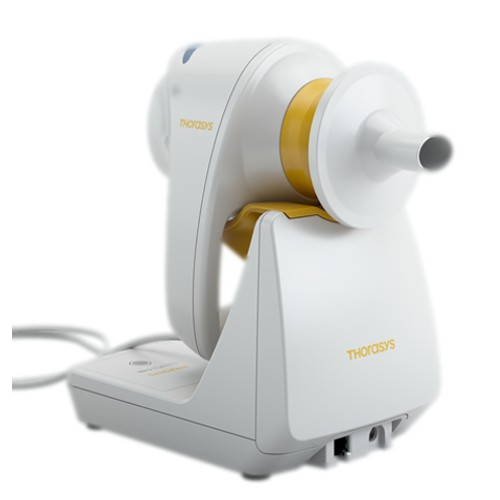
\includegraphics[width=0.7\textwidth]{tremoflo}
			\caption{Přístroj Tremoflo C-100 \cite{wwwpics}}
			 \label{tremoflopristroj}
 \end{figure}

Přístroj je kompaktní a přenosný. TremoFlo a jeho software jsou pro uživatele velmi přístupné a intuitivní. Měření je velmi rychlé (proběhne v rámci několika minut). UI softwaru nám poskytuje obraz měřených dat v reálném čase, přičemž jejich finální zpracování je vysoce detailní. Program též zaznamenává a zapisuje do své databáze výsledky měření jednotlivých pacientů.

Software pro analýzu dat z přístroje je velmi uživatelsky přístupný. 

\begin{figure}[!ht]
			\centering
 			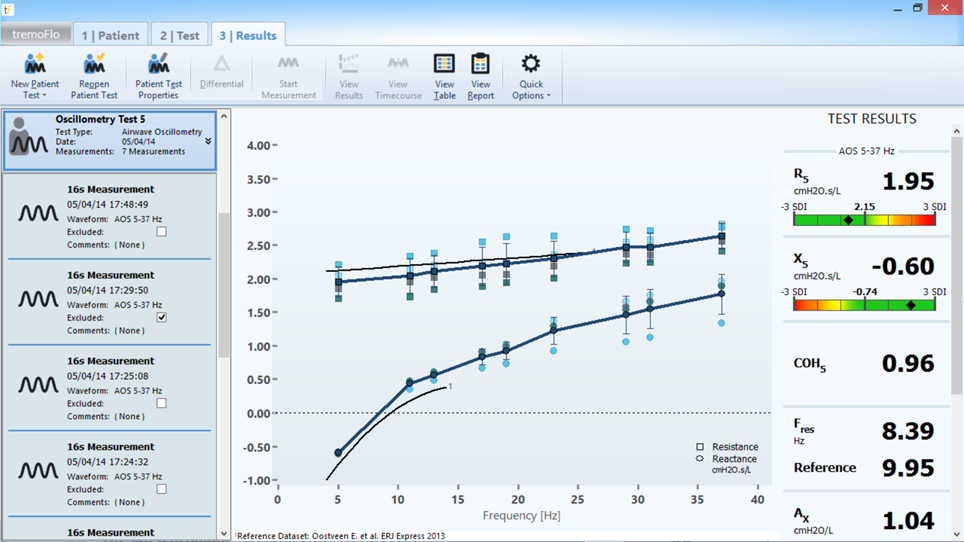
\includegraphics[width=1\textwidth]{sw}
			\caption{Obrazovka ovládacího software \cite{wwwpics}}
			 \label{tremosw}
 \end{figure}

Další z~přístrojů využívající metodu nucených oscilací je například PulmoScan. Hlavní rozdíl přístrojů PulmoScan a Tremoflo C-100 je absence nutnosti drátového připojení. 